\documentclass[a4paper,12pt]{article}
\usepackage[utf8]{inputenc}
\usepackage[lmargin=2.5cm,rmargin=2.5cm,tmargin=2.5cm,bmargin=2.5cm]{geometry}
\usepackage{amsmath,amsthm,amssymb}
\usepackage{hyperref}
\usepackage{todonotes}

\usepackage{graphicx}

\setlength\parindent{0pt}

\begin{document}


\subsection*{Mapping public keys into a colored circle}

\textit{Problem}: encode (part of) a public key given in hex in a colored circle via a unique mapping.\\

\textit{Idea}: 
Assume the circle has length N and we have $C \geq N$ colors used for the $K \in \{2,...N\}$ segments of the circle, then we can simply count all possible, colored circles that can be generated and assign in a deterministic way an index. Mapping our hex key to an integer will then give us an index that corresponds one-to-one to a colored circle.\\

First, we assume that K is fixed.
We can count the number of ways to group $N$ pieces of the circle into $K$ segments by treating it as a stars and bars problem (see \href{https://en.wikipedia.org/wiki/Stars_and_bars_(combinatorics)}{here}). There are ${N-1 \choose K-1}$ ways to group them. This will be useful later.
We can also count the number of ways to color K segments with C colors. In our case we don't want duplicates. So we can just take a permutation. So there are $P(C,K)$ ways to color the K segments.
Combining this, in total there are ${N-1 \choose K-1} \cdot P(C,K)$ total circles for a circle with $N$ pieces being grouped into $K$ segments that can be colored with $C$ colors.

So given a number in $ [ 0,..., {N-1 \choose K-1} \cdot P(C,K) ] $, we can first decompose it into two numbers in the ranges $[0,..., {N-1 \choose K-1}]$ and $[0,..., P(C,K)]$ respectively. These are our ranks for the segment grouping and the coloring.\\
    
\textbf{Ranks for segment grouping:} We can begin to unrank the segment grouping by treating it as a stars and bars problem. We just need a way to go from a rank to a permutation. There are algorithms for generating all the permutations in lexicographic order. The one we're interested in Narayana Pandita's generation algorithm (see \href{https://en.wikipedia.org/wiki/Permutation#Generation_in_lexicographic_order}{here}). We can reverse this algorithm to go from a rank to a permutation which gives us the segments of our circle.\\
    
 \textbf{Ranks for coloring:} $P(C,K)$ is defined as the product of $\{C, C-1, ..., C - K + 1\}$. The set $[0,...,P(C,K)]$ give us our color indices if we decompose them from the rank. Since we need to avoid repetition of color, this will give us a list of color indexes that are a little off. For instance if we got [0, 0] as our indexes, this would mean the 0th color and the 1st color. Because the second index assumes the first index was removed from the list. So once we extract the color indices, we need to adjust them with the assumption that every previously extracted index was removed.\\
    
\textbf{Summary for fixed K:} Combining what we described so far, given a number in hex, we map it to an integer $X$ in $[0,..{N-1 \choose K-1} \cdot P(C,K)]$. We then extract the segment rank $A$ by using $X \ \text{mod} \ {N-1 \choose K-1}$ to get a number in the range $[0,..., {N-1 \choose K-1}]$. The coloring rank $B$ is extracted using $\lfloor X \div {N-1 \choose K-1} \rfloor $. From here we use our reverse permutation algorithm to determine the star and bars permutation that the rank corresponds to. And we further decompose our coloring rank into numbers in the ranges $\{[0,...,C], [0,...,C-1], ..., [0,...,C - P + 1]\}$ like we did before. Finally we adjust those indices to account for the assumption that every previous index is removed. This leaves us with every index in the range $[0,...,C]$ which is our color indices.\\

\textbf{Final Step for varying K:} This is how you would map a number to a circle with only one $K$ value. To map to a range of K values, a small step is required before the above steps. We need to calculate the amount of circles for each K value we're interested in. From there we can add them all up to be our total circle count $R_T$. The numbers in the range $[0,...,R_T]$ can be split into chunks of lengths $[R_1, R_2, ..., R_K]$ where each $R$ value is another circle count for a certain segment count. In our case, the first chunk corresponds to the K = 2, the second chunk corresponds to K = 3, and so on. Now when an index falls in one of these ranges, we map the lowest index to 0 and then proceed with the steps we outlined above.\\

\textbf{Easy Example:}
Let us assume we have a circle of length $N=3$, we split it into $K \in \{1,2,3\}$ segments and we have $C=5$ colors, which are given in a ordered set (i.e. blue is one, red is two, and so on).
Then for $K=1$, we get 5 different circles.
For $K=2$, we get $ 40 (=2 \cdot 20)$ different colored circles.
For $K=3$, we have $60 (=1 \cdot 60)$ unique colored circles.
In total, we have $105$ different circles.

Now, given an integer $X \in \{0,...104\}$, we proceed as follows:
\begin{enumerate}
    \item Check in which range we are and choose the number of segments accordingly.\\ If $X \in \{0,..,4\}$, $K=1$,\\ else if $X \in \{5, ... 44\}$, $K=2$\\ and if $X \in \{ 45, ..., 105\}$ we get $K=3$.
    \item For K=1, we proceed as follows: since we only have one segment, there is only one segmentation and only the coloring is meaningful. Hence, we simply assign each number in \{0,..,4\} the corresponding color from the given set of ordered colors.
    \item For K=2, we first need to choose the right segmentation. We take $X \ \text{mod} \ {2 \choose 1} = X \ \text{mod} \ 2$ to choose from the two possible segmentation (in this case[(1,2),(2,1)]). For the coloring we calculate $\lfloor X \div {2 \choose 1} \rfloor = \lfloor X \div 2 \rfloor $, which gives a number from 2 to 22. Next step is the coloring, for which we map the first number 2 to the coloring (C1, C2), the second to (C1,C3) and iterate through the tuples of colors (excluding the repetition of colors).
    \item For $K=3$, we proceed as for $K=2$ and map our number to a unique circle with 3 colors.
\end{enumerate}

\begin{figure}[h!]
    \centering
    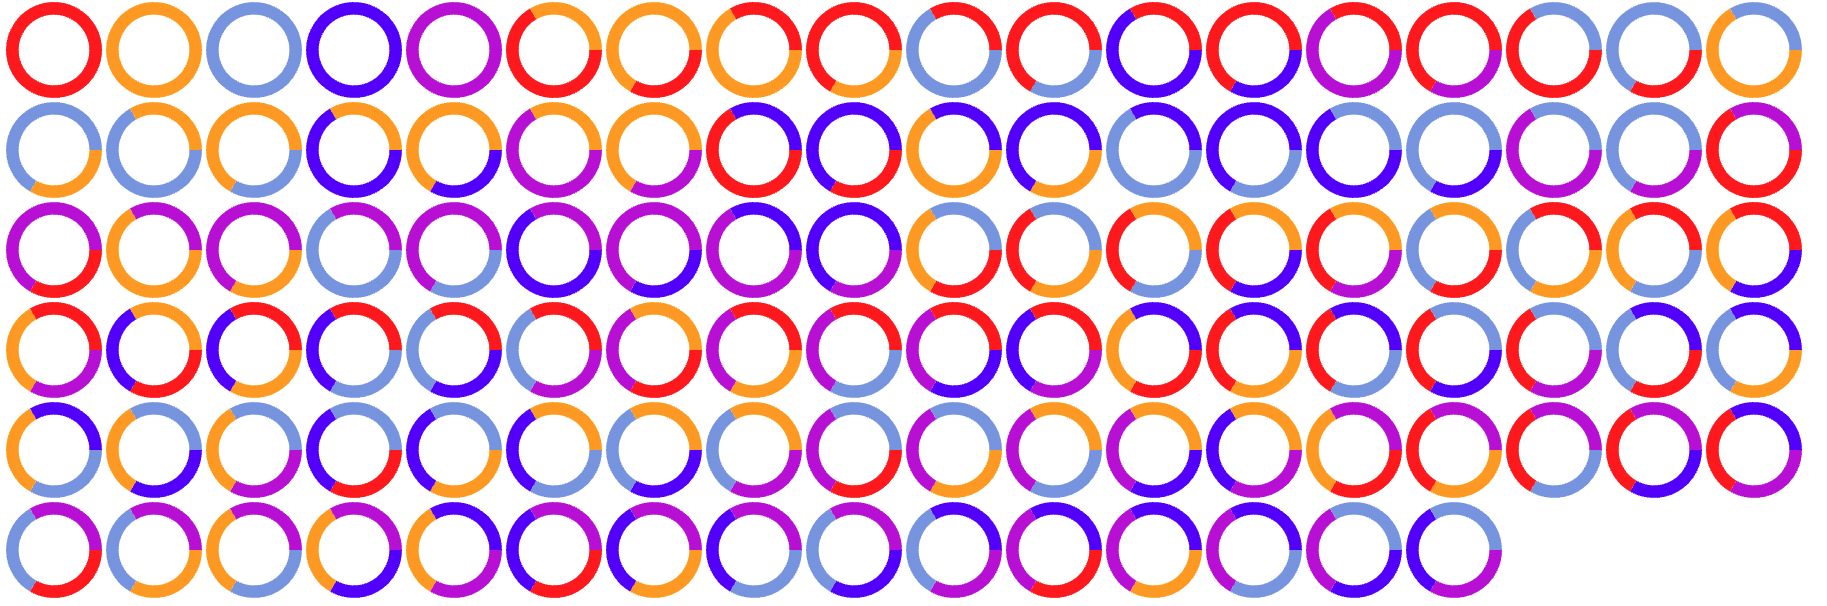
\includegraphics[keepaspectratio, width = 12cm]{circles_example.png}
    \caption{Example with 105 circles and parameters length N=3, colors C=5 and 1 to 3 segments K.}
\end{figure}

%%%%%%%%%%%%%%%%%% new page 
\newpage
\section*{Parameter analysis of a secure map of status.im public keys}

The purpose of the this document to provide a brief analysis of given options to securely map status.im 512 bit chat keys/public keys to a different encoding, leveraging a combination of emojis and colors (and optionally additional factors) to encode the key.\\

\subsection*{Mapping public keys into two alphabets}
\noindent Given a key of 512 bit-length, we can map this key to a different representation:

\begin{equation}
    M: [0,1]^{512} \rightarrow [0,1024]^{n}  \times [0,32]^{k} 
\end{equation} 
with n and k integers.\\


\noindent To ensure the mapping doesn't break the security of the overall scheme, it needs to be bijective. We need to choose n and k accordingly:

\begin{align}
    2^{512} & = 1024^n \cdot 512^k \\
    2^{512} & = (2^{10})^n \cdot (2^5)^k \\
    2^{512} & = 2^{10 \cdot n + 5 \cdot k}
\end{align}
and taking $log_2$ on both sides gives us
\begin{align}
    512 & = 10 \cdot n + 5 \cdot k
\end{align}

\noindent Whereas in bit-representation, our key has 512 characters, this number is reduced by the mapping M. If we map it to 0x, we need 128 chars. The challenge is to define a mapping that yields significant compression. If we only take one representation on the right hand side, we reduce the representation to roughly 52 for k=0 (only emojis) or 103 for n=0 (only colors).\\


\noindent Combining both representations, we get a trade-off between the large one and the smaller one. In our case, this is

\begin{align}
    n & = \frac{512}{10} - \frac{k}{2}
\end{align}
hence, \textbf{increasing k by 2 leads to a reduction in n by only 1.}\\


\noindent To illustrate this, let us start from $k=0$ (colors). Then we need $n=52$ (emojis). Increasing now $k$ to $10$, we still need roughly $n=47$. For $k = 20$, we need $n = 42$ and for $k = 30$ we get $n = 37$.\\

\noindent Note that since n and k need to be integers, we sometimes have to round them up to ensure that our mapping can be bijective.





\end{document}